\documentclass[a4paper]{article}
\usepackage{eacl2012}
\usepackage{url}
\usepackage{graphicx}
\usepackage{qtree}
\usepackage{ccg}
\usepackage{subfig}
\usepackage{tikz}
\usepackage{amsmath}

% use this macro to hide things for anonymous review
\newcommand\anonymize[1]{}
%\renewcommand\anonymize[1]{#1} % uncomment to de-anonymize

\author{
\anonymize{
Jonathan Weese \and Chris Callison-Burch \and Adam Lopez\\
Department of Computer Science\\
Human Language Technology Center of Excellence\\ % are we all in HLTCOE, or just Chris and Adam?
Johns Hopkins University\\
Baltimore, MD 21218 USA\\
{\tt \{jonny,ccb,alopez\}@cs.jhu.edu}}
}
\title{Label Elegance in Statistical Machine Translation}

\begin{document}
\maketitle

\begin{abstract}
Adding syntactic labels to synchronous context-free translation rules can improve performance, but only using phrase structure constituents, as in GHKM \cite{ghkm}, excludes potentially useful translation rules. SAMT \cite{samt-wmt06} introduces heuristics to create new non-constituent labels, but these heuristics introduce many complex labels and tend to add rarely-applicable rules to the translation grammar. We introduce a new labeling scheme based on categorial grammar, which allows syntactic labeling of many rules with a minimal, well-motivated label set. We show that our labeling scheme performs comparably to SAMT on an Urdu--English translation task, yet the label set is an order of magnitude smaller, and translation is twice as fast.
\end{abstract}

\section{Introduction}

The Hiero model of \newcite{Chiang2007} popularized the usage of synchronous context-free grammars (SCFGs) for machine translation. SCFGs model translation as a process of isomorphic syntactic derivation in the source and target language. But the Hiero model is formally, not linguistically syntactic. Its derivation trees carry only a single non-terminal label $X$, carrying no linguistic information. Consider Rule \ref{eqn:hiero}.
\begin{equation}
X \to \langle \textrm{ maison ; house } \rangle\label{eqn:hiero}
\end{equation}

We may try to add syntactic information to the SCFG rules by parsing the parallel training data and projecting that information down. For example, if we knew from a phrase structure parse that {\em house} was a noun, we could rewrite Rule \ref{eqn:hiero} as
\begin{equation*}
N \to \langle \textrm{ maison ; house } \rangle
\end{equation*}

But we quickly run into trouble: how should we label a rule that translates {\em pour l'\'{e}tablissement de} into {\em for the establishment of}? There is no phrase structure constituent that corresponds to this English fragment.

We could simply throw away any rules that can't be labeled syntactically, but that hurts translation performance \cite{koehn-och-marcu-2003,deneefe-syntax-and-phrase-mt}.

Syntax-Augmented Machine Translation 
(SAMT; Zollmann and Venugopal, 2006) \nocite{samt-wmt06} % stupid style file is stupid; should work with \cite[before text][after text]{citename} but doesn't
solves this problem with heuristics that create new labels from the phrase structure parse: it labels {\em for the establishment of} as IN+NP+IN to show that it is the concatenation of a noun phrase with a preposition on either side. While descriptive, this label is dissatisfying as a concise description of linguistic function, fitting uneasily alongside more natural labels in the phrase structure formalism. SAMT introduces many thousands of such labels, most of which are seen very few times. While these heuristics are effective \cite{zollmann+etal:2008:coling}, they inflate grammar size, hamper effective parameter estimation due to feature sparsity, and slow translation speed.

We would like to find another syntactic formalism that will allow us to label most translation rules without relying on heuristics. Further, we'd like the label set to be small in order to improve feature estimation and reduce translation time. We show that {\em combinatory categorial grammar} (CCG) satisfies these requirements.

Under CCG, {\em for the establishment of} is labeled with ((S\textbackslash NP)\textbackslash (S\textbackslash NP))/NP. This seems complex, but it describes exactly how the fragment should combine with other English words to create a complete sentence in a linguistically meaningful way. We show that CCG is a viable  formalism to add syntax to SCFG-based translation.

%%% THIS IS THE OLD INTRODUCTION
%
%Synchronous context-free grammars (SCFGs) were popularized for statistical machine translation by Chiang with his Hiero model \shortcite{chiang2005}. An SCFG is used to define translation rules that may have gaps in them.
%As an example, consider the rule
%\begin{equation}
%X \to \langle \textrm{ do not } X_1 ; \textrm{ ne } X_1 \textrm{ pas } \rangle \label{rule:ne_pas}
%\end{equation}
%This rule encodes the idea that the English phrase {\em do not X} can be translated into French {\em ne X pas}, as long as the $X$ phrases are themselves translation pairs. (The correspondence between the two $X$s on the right-hand side of the rule is shown by their subscripts.)

%So if we are given another rule
%\begin{equation}
%X \to \langle \textrm{ house ; loge } \rangle
%\end{equation}
%where ``house'' is used in the sense of the verb ``to shelter something'' we can conclude that {\em do not house} should be translated into {\em ne loge pas}.

%The rules above are typical of the Hiero model, where all non-terminal labels have the same symbol ($X$). However, this simple model has drawbacks. Since every non-terminal is an $X$, every phrase may theoretically fit into any slot. If we were given a (more common) Hiero rule for the noun ``house''
%\begin{equation}
%X \to \langle \textrm{ house , maison } \rangle
%\end{equation}
%we could form the French translation {\em ne maison pas}. 
%
%We know that Rule \ref{rule:ne_pas} should only be applied when the missing phrase is a verb, but Hiero does not include any information about the syntactic type of rules or their missing phrases.
%
%To improve this SCFG model, we want to assign labels to the rules that describe their syntactic roles. However, if the set of labels is too restrictive, we may not be able to label all translation rules. These non-syntactic rules are essential to translation performance in both phrase-based \cite{koehn-och-marcu-2003} and syntactic MT models \cite{deneefe-syntax-and-phrase-mt}.
%
% We might try to assign syntactic labels by reading them from a phrase structure parse of the training data: assign labels from the parse tree where possible, and throw out all other translation rules. However, translation rules that don't correspond to these syntactic forms are essential to translation performance in both phrase-based \cite{koehn-och-marcu-2003} and syntactic MT models \cite{deneefe-syntax-and-phrase-mt}.
%
%Syntax-augmented Machine Translation (SAMT) \cite{samt-wmt06} increases rule coverage by using heuristics to assign complex labels to rules. %: if a rule can't be assigned a simple syntactic form, we may assign a new label by concatenating labels or by introducing {\em slashed} labels for incomplete rules.
%SAMT improved performance over other syntactic models, but the heuristic label set violates some principles about what a syntactic labeling scheme should look like:
%
%The label set should be well-motivated: the labels should represent actual syntactic structure under some accepted model of syntax. The label set should also be small: a smaller non-terminal set allows for better estimation of features that depend on these labels, and keeps translation efficient. 
%\begin{itemize}
%\item The concatenated and slashed labels are not common linguistic labels; they're introduced solely to increase the number of extractable rules.
%\item The number of rules in the grammar and the size of the non-terminal set are both significantly larger than their Hiero or GHKM counterparts.
%\item Because of the larger model size, translation speed decreases significantly.
%\end{itemize}
%
%Ideally, we'd like to find a rule labeling strategy that is linguistically well-motivated, uses a smaller label set than SAMT, but still allows many useful translation rules to be extracted.
%
%, we can devise a set of labels that satisfy these principles and still allow many translation rules to be extracted.
\begin{itemize}
\item We introduce two models for labeling SCFG rules. One uses labels from a 1-best CCG parse tree of training data; the second uses the top labels in each cell of a CCG parse chart.
\item We show that using 1-best parses performs as well as a syntactic model using phrase structure derivations.
\item We show that using chart cell labels performs almost as well than SAMT, but the non-terminal label set is an order of magnitude smaller and translation is twice as fast.
\end{itemize}

\section{Categorial grammar}
\label{sec:cg}

Categorial grammar (CG) \cite{cg,bar-hillel-cg} is a grammar formalism in which words are assigned grammatical types, or {\em categories}. Once categories are assigned to each word of a sentence, a small set of universal combinatory rules uses them to derive a sentence-spanning syntactic structure.

Categories may be either atomic, like N, VP, S, and other familiar types, or they may be complex {\em function types}. A function type looks like A/B and takes an of type B and returns a type A. The categories A and B may themselves be either primitives or functions. A lexical item is assigned a function category when it takes an {\em argument} --- for example, a verb may be function that needs to be combined with its subject and object, or an a adjective may be a function that takes the noun it modifies as an argument.

We can combine two categories with {\em function application}. Formally, we write
\begin{equation}
%A/B \, B \to A 
\binaryruleSimple{X/Y}{Y}{X}\label{eqn:forward-app}
\end{equation}
to show that a function type may be combined with its argument type to produce the result type.

Combinatory categorial grammar (CCG) is an extension of CG that includes more {\em combinators} (operations that can combine categories). Steedman and Baldridge \shortcite{ccg} give an excellent overview of CCG.

As an example, suppose we want to analyze the sentence ``They own properties in various cities and villages'' using the lexicon shown in Table \ref{table:lexicon}. We assign categories according to the lexicon, then combine the categories using function application and other combinators to get an analysis of S for the complete sentence. Figure \ref{fig:ccg-derivation} shows the derivation tree.

\begin{table}
\centering
\begin{tabular}{|c|c|}
\hline
Lexical item & Category \\
\hline
and & conj \\
cities & NP \\
in &  (NP\textbackslash NP)/NP \\
own & (S\textbackslash NP)/NP \\
properties & NP \\
they & NP \\
various & NP/NP \\
villages & NP \\
\hline
\end{tabular}
\caption{An example lexicon, mapping words to categories.\label{table:lexicon}}
\end{table}

\begin{figure*}
\centering
\deriv{8}{
They & own & properties & in & various & cities & and & villages \\
\uline{1} & \uline{1} & \uline{1} & \uline{1} & \uline{1} & \uline{1} & \uline{1} & \uline{1} \\% & \uline{1} \\
NP & (S\backslash NP)/NP & NP & (NP\backslash NP)/NP & NP/NP & NP & conj & NP \\%& ((S\backslash NP)/(S\backslash NP))/NP & N/N & N \\
& & & & \fapply{2} & \conj{2} \\
& & & & \cmc{2}{NP} & \cmc{2}{NP\backslash NP} \\
& & & & \bapply{4} \\
& & & & \cmc{4}{NP} \\
& & & \fapply{5} \\
& & & \cmc{5}{NP\backslash NP} \\
& & \bapply{6} \\
& & \cmc{6}{NP} \\
& \fapply{7} \\
& \cmc{7}{S\backslash NP} \\
\bapply{8} \\
\cmc{8}{S}
}
\caption{An example CCG derivation for the sentence ``They own properties in various cities and villages'' using the lexicon from Table \ref{table:lexicon}. $\Phi$ indicates a conjunction operation; $>$ and $<$ are forward and backward function application, respectively.\label{fig:ccg-derivation}}
\end{figure*}

As we will show, the labels that CCG derives for each span of the sentence meet the criteria we listed at the beginning of this section:
\begin{enumerate}
\item They naturally provide labels for many more spans of an input sentence than a phrase structure parse does.
\item Despite this increase in labeled spans, the set of categories remains small and linguistically meaningful.
\end{enumerate}

\subsection{Labels for phrases}

The motivation for assigning new labels to translation rules is to annotate the rules with syntactic information. But this raises a design question: what label do we assign to spans that are natural translations of each other, but have no natural labeling under a syntactic parse?
One possibility would be to discard such translations from our model as implausible. However, such non-compositional translations are important in translation \cite{fox:2002:emnlp}, and it has been repeatedly shown that discarding potential translation rules because they do not correspond to full syntactic constituents is harmful for translation performance under a variety of models \cite{koehn-och-marcu-2003,deneefe-syntax-and-phrase-mt} 

Consider for example the German--English phrase pair {\em  -- the tall man}. It is easily labeled as an NP and included in the translation table. By contrast, {\em -- the tall}, doesn't typically correspond to a complete subtree in a phrase structure parse. Yet translating {\em the tall} is likely to be useful than translating {\em the tall man}, since it is more general---it can be combined with any other noun translation.

Using CG-style labels with function types, we can assign the type (for example) NP/N to {\em the tall} to show that it can be combined with a noun on its right to create a complete noun phrase.\footnote{We could assign NP/N to the determiner {\em the} and N/N to the adjective {\em tall}, then combine those two categories using {\em function composition} to get a category NP/N for the two words together.}

More generally, CG labels can be used annotate syntax of almost any span, while still remaining linguistically meaningful.

\subsection{Minimal, well-motivated label set}

By allowing slashed categories with CG, we're increasing the number of labels allowed. There are other ways to create new syntactic labels for phrases like {\em the tall}, but CG is the best way for two reasons:
\begin{enumerate}
\item CG labels are well-motivated. Our labels are derived from CCG derivations, so phrases with slashed labels {\em really are} labeled that way in a syntactic formalism, and the categories can be naturally combined.
\item The set of labels is still small --- it's restricted to the labels seen in CCG parses of the training data.
\end{enumerate}

Another way to grow the label is set is to use the strategy of the Syntax-Augmented Machine Translation model (SAMT) \cite{samt-wmt06}. SAMT allows arbitrary concatenation of labels and arbitrary ``slashing.'' For example, exactly one rule in the SAMT grammar was labeled with ,+WDT+VBN --- a comma followed by a WH-determiner followed by a past participle verb. This greatly increases the size of the label set, and adds a lot of labels are only seen once in the entire grammar. This causes problems both for feature estimation (since label counts are now sparse) and for decoding time (since the non-terminal set affects the grammar constant for parsing --- see Section \ref{sec:comparison}).

In short, using CG labels allows us to keep more syntactic rules without making the set of syntactic labels too big.

\section{Translation models}

\subsection{Synchronous context-free grammars}

Formally, an SCFG may be defined as a 5-tuple
$$(N,S,T_\sigma,T_\tau,G)$$
where $N$ is a set of non-terminal symbols, $S \in N$ is a distinguished start symbol, $T_\tau$ and $T_\sigma$ are the source- and target-side terminal symbol vocabularies, and $G$ is a set of production rules. Each rule in $G$ is of the form
$$X \to \langle \alpha, \gamma, \sim \rangle$$
where $X \in N$, $\alpha$ is a sequence of symbols drawn from $N \cup T_\sigma$, $\gamma$ is a sequence of symbols drawn from $N \cup T_\tau$, and $\sim$ is a one-to-one correspondence between the terminal symbols in $\alpha$ and $\gamma$.

We may define several {\em feature functions} $\phi_i$ on rules in $G$, and assign each feature a weight $\lambda_i$. Then the {\em weight} of a rule in $G$ is
\begin{equation}
w(r) = \prod_i{\phi_i(r)^{\lambda_i}}
\end{equation}

The weight assigned to a derivation under this SCFG is the product of the weights of the rules used; that is, for some derivation $D$,
\begin{equation}
w(D) = \prod_{r \in D}{w(r)}
\end{equation}

To translate a sentence under an SCFG model, we parse an input sentence $f$ to generate translation candidates --- the set of candidates is exactly the set of strings $e$ such that the pair $(f,e)$ is licensed by the SCFG.

For each candidate $e$, the weight of its derivation is just one of the features that may be added to a log-linear model to determine the most likely translation.

\subsection{Extraction from parallel text}

\begin{figure}[t]
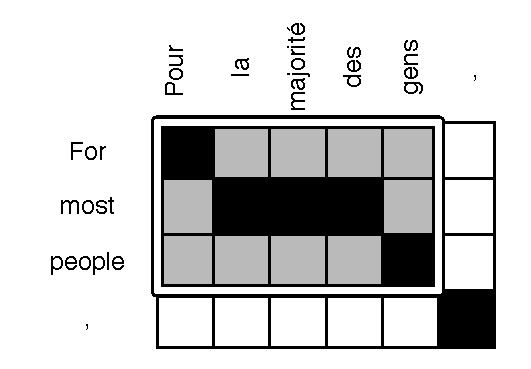
\includegraphics[width=0.4\textwidth]{figures/simple-rule}
\caption{A word-aligned sentence pair fragment, with a box indicating a consistent phrase pair.\label{fig:aligned-sentence}}
\end{figure}

\begin{figure}[t]
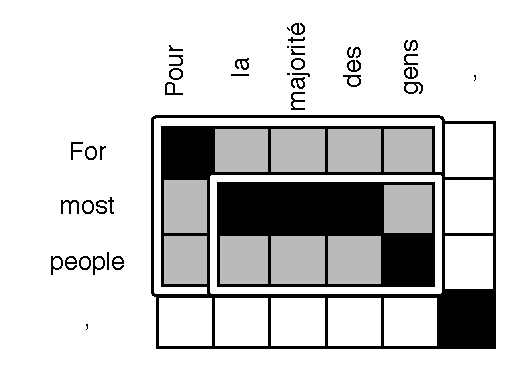
\includegraphics[width=0.4\textwidth]{figures/hierarchical-rule}
\caption{A consistent phrase pair with a sub-phrase that is also consistent. We may extract a hierarchical SCFG rule from this training example.\label{fig:hierarchical-phrases}}
\end{figure}

To extract SCFG rules, we start with a heuristic to extract phrases from a word-aligned sentence pair \cite{tillmann-2003}. Figure \ref{fig:aligned-sentence} shows a such a pair, with a {\em consistent phrase pair} inside the box. A phrase pair $(f,e)$ is said to be consistent with the alignment if none of the words of $f$ are aligned outside the phrase $e$, and vice versa -- that is, there are no alignment points directly above, below, or to the sides of the box defined by $f$ and $e$.

Given a consistent phrase pair, we can immediately extract the rule
\begin{equation}
X \to \langle f , e \rangle
\end{equation}
as we would in a phrase-based MT system. However, whenever we consistent phrase pair that is a sub-phrase of another (see Figure \ref{fig:hierarchical-phrases} for an example), we may extract a hierarchical rule by treating the inner phrase as a gap in the larger phrase. For example, we may extract the rule
\begin{equation}
X \to \langle \textrm{ Pour X }; \textrm{ For X } \rangle
\label{eqn:hiero-rule}
\end{equation}
from Figure \ref{fig:hierarchical-phrases}.

The focus of this paper is how to assign labels to the left-hand non-terminal $X$ and to the non-terminal gaps on the right-hand side. We discuss five models below, of which two are novel CG-based labeling schemes.

\subsection{Baseline: Hiero}

Hiero \cite{Chiang2007} uses the simplest labeling possible: there is only one non-terminal symbol, X, for all rules.  Its advantage over phrase-based translation in its ability to model phrases with gaps in them, enabling phrases to reorder subphrases. However, since there's only one label, there's no way to include syntactic information in its translation rules.

\subsection{Phrase structure parse tree labeling}

One first step for adding syntactic information is to get syntactic labels from a phrase structure parse tree. For each word-aligned sentence pair in our training data, we also include a parse tree of the target side.

Then we can assign syntactic labels like this: for each consistent phrase pair (representing either the left-hand non-terminal or a gap in the right hand side) we see if the target-language phrase is the exact span of some subtree of the parse tree.

If a subtree exactly spans the phrase pair, we can use the root label of that subtree to label the non-terminal symbol. If there is no such subtree, we throw away any rules derived from the phrase pair.

As an example, suppose the English side of the phrase pair in Figure \ref{fig:hierarchical-phrases} is analyzed as
\begin{center}
\Tree [.PP [.IN For ] [.NP [.JJ most ] [.NN people ] ] ]
\end{center}
Then we can assign syntactic labels to Rule \label{eqn:hiero-rule} to produce
\begin{equation}
\textrm{PP } \to \langle \textrm{ Pour NP }; \textrm{ For NP } \rangle
\end{equation}

The rules extracted by this scheme are very similar to those produced by GHKM \cite{ghkm}, in particular resulting in the "composed rules" of \newcite{ghkm-scalable-inference}, though we use simpler heuristics for handling of unaligned words and scoring in order to bring the model in line with both Hiero and SAMT baselines.
As we noted in Section \ref{sec:cg}, under this scheme we may throw away a lot of useful translation rules that don't translate exact syntactic constituents. We can alleviate this problem by changing the way we get syntactic labels from parse trees.

\subsection{SAMT}

The Syntax-Augmented Machine Translation (SAMT) model \cite{samt-wmt06} extracts more rules than the other syntactic model by allowing different labels for the rules. In SAMT, we try several different ways to get a label for a span, stopping the first time we can assign a label:
\begin{itemize}
\item As in simple phrase structure labeling, if a subtree of the parse tree exactly spans a phrase, we assign that phrase the subtree's root label.
\item If a phrase can be covered by two adjacent subtrees with labels A and B, we assign their concatenation A+B.
\item If a phrase spans part of a subtree labeled A that could be completed with a subtree B to its right, we assign A/B.
\item If a phrase spans part of a subtree A but is missing a B to its left, we assign A\textbackslash B.
\item Finally, if a phrase spans three adjacent subtrees with labels A, B, and C, we assign A+B+C.
\end{itemize}
Only if all of these assignments fail do we throw away the potential translation rule.

We note here that the slashed labels of SAMT are inspired by CCG, but they're not the same as our slashed labels: CCG function categories are used for syntactic structures that take arguments, like adjectives or verbs, but the SAMT slashed labels simply denote incomplete syntactic constituents.

\subsection{CCG 1-best derivation labeling}

Our first CG model is similar to the first phrase structure parse tree model. We start with a word-aligned sentence pair, but we parse the target sentence using a CCG parser instead of a phrase structure parser.

When we extract a rule, we see if the consistent phrase pair is exactly spanned by a category generated in the 1-best CCG derivation of the target sentence. If there is such a category, we assign that category label to the non-terminal. If not, we throw away the rule.

To continue our extended example, suppose the English side of Figure \ref{fig:hierarchical-phrases} was analyzed by a CCG parser to produce
\begin{center}
\deriv{3}{
For & most & people \\
\uline{1} & \uline{1} & \uline{1} \\
(S/S)/N & N/N & N \\
& \fapply{2} \\
& \cmc{2}{N} \\
\fapply{3} \\
\cmc{3}{S/S}
}
\end{center}
Then just as in the phrase structure model, we project the syntactic labels down onto the extractable rule yielding
\begin{equation}
\textrm{S/S } \to \langle \textrm{ Pour N }; \textrm{ For N } \rangle
\end{equation}

This does not take advantage of CCG's ability to label almost any fragment of language: the fragments with labels in any particular sentence depend on the order that categories were combined in the sentence's 1-best derivation. In the next model, we increase the number of spans we can label.

\subsection{CCG parse chart labeling}

In the first CCG model, we use the 1-best CCG derivation to assign labels to spans. This means that a lot of possible rules can't be labeled, because their phrase pairs don't match up to a span in the particular derivation tree.

For this model, we do not use the 1-best CCG derivation. Instead, when parsing the target sentence, for each cell in the parse chart, we read the most likely label according to the parsing model. This lets us assign a label for almost any span of the sentence just by reading the label from the parse chart.

Thus, when we want to assign a label to a non-terminal on the left- or right-hand side of a rule, we determine what part of the target sentence that the non-terminal spans. Since we've read the 1-best category label from each cell of the parse chart, we have a category for every possible span of the sentence.

\section{Comparison of resulting grammars}
\label{sec:comparison}

Our labeling schemes are trying to satisfy two competing desires: first, we want to keep as many rules as possible, knowing that some of them will turn out to be useful in translation. Thus we want to add syntactic labels until we can label everything. On the other hand, large labeling sets lead to problems:
\begin{enumerate}
\item For a rule $A \to \langle f ; e \rangle$, we may want to estimate feature scores that condition on the syntactic type, such as $p(e|A)$ and $p(f|A)$. Sparse counts will make it hard to estimate this probability correctly.
\item If an otherwise-useful translation rule is assigned a rare syntactic type, it will be used less often in translations. This is because there will be few other translation rules that expect a phrase of that type to fill a gap.
\end{enumerate}
What we would like is a relatively constrained non-terminal label set, so that we can estimate features with confidence, and so that translation rules have a chance of being used in more derivations. But we want the label set to be general enough that we don't throw away any more translation rules than we have to.


\subsection{Effect of grammar size and label set on parsing efficiency}

There are sound theoretical reasons for reducing the number of non-terminal labels in a grammar. Translation with a synchronous context-free grammar requires first parsing with the source-language projection of the grammar, followed by intersection of the target-language projection of the resulting grammar with a language model. While there are many possible algorithms for these operations, they all depend on the size of the grammar.

Consider for example the popular cube pruning algorithm of Chiang
\shortcite{Chiang2007}, which is a simple extension of CKY. It works by first
constructing a set of items of the form $\langle A, i, j \rangle$,
where each item corresponds to (possibly many) partial analyses by
which nonterminal $A$ generates the sequence of words from positions
$i$ through $j$ of the source sentence. It then produces an augmented
set of items $\langle A, i, j, u, v \rangle$, in which items of the
first type are augmented with left and right language model states $u$
and $v$. In each pass, the number of items is linear in the number of
nonterminal symbols of the grammar. This observation has motivated
work in grammar transformations that reduce the size of the
nonterminal set, often resulting in substantial gains in parsing or
translation speed \cite{song2008,denero-efficient-parsing,xiao2009}.

More formally, the upper bound on parsing complexity is always at
least linear in the size of the grammar constant $G$, where $G$ is
often loosely defined as a {\it grammar constant}; Iglesias et al.
\shortcite{iglesias2011} give a nice analysis of the most common translation algorithms
and their dependence on $G$. Dunlop et al. \shortcite{dunlop2010} provide a more
fine-grained analysis of $G$, showing that for a variety of
implementation choices that it depends on either or both the number of
rules in the grammar and the number of nonterminals in the grammar.
Though these are worst-case analyses, it should be clear that grammars
with fewer rules or nonterminals can generally be processed more
efficiently.

\subsection{Number of rules and non-terminals}

Table \ref{table:rule-count} shows the number of rules we can extract under various labeling schemes. The rules were extracted from an Urdu--English parallel corpus with 202,019 translations, or almost 2 million words in each language.

As we described before, moving from the phrase-structure syntactic model to the extended SAMT model vastly increases the number of translation rules --- from about 7 million to 40 million rules. But the increased rule coverage comes at a cost: the non-terminal set has increased in size from 70 (the size of the set of Penn Treebank tags) to over 18,000.

Comparing the phrase structure syntax model to the 1-best CCG derivation model, we see that the number of extracted rules increases slightly, and the grammar uses a set of about 500 non-terminal labels. This does not seem like a good trade-off; since we are extracting from the 1-best CCG derivation there really aren't many more rules we can label than with a 1-best phrase structure derivation.

But when we move to the full CCG parse chart model, we see a significant difference: when reading labels off of the entire parse chart, instead of the 1-best derivation, we don't see a significant increase in the non-terminal label set. That is, most of the labels we see in parse charts of the training data already show up in the top derivations: we're not making up new labels that have never been seen before.

But by using the chart cells, we are able to assign syntactic information to many more translation rules: over 28 million rules, for a grammar about $\frac{3}{4}$ the size of SAMT's. The parse chart lets us extract many more rules without significantly increasing the size of the syntactic label set.

\begin{table}
\centering
\begin{tabular}{|c|r|r|}
\hline
Model & Rules & NTs\\
\hline
Hiero & 4171473 & 1\\
Syntax & 7034393 & 70\\
SAMT & 40744439 & 18368\\
CG Model 1 & 8042683 & 505\\
CG Model 2 & 28961161 & 517\\
\hline
\end{tabular}
\caption{Number of translation rules and non-terminal labels in an Urdu--English grammar under various models.\label{table:rule-count}}
\end{table}

%\begin{table}
%\centering
%\begin{tabular}{|c|c|c|}
%\hline
%Model & Non-terminal labels & Singletons \\
%\hline
%Hiero & 1 & 0 \\
%Syntax & 70 & 0 \\
%SAMT & 18368 & 883 \\
%CG Model 1 & 505 & 25 \\
%CG Model 2 & 517 & 36 \\
%\hline
%\end{tabular}
%\caption{Number of non-terminal labels present in an Urdu--English grammar for various models. A singleton label is a label that only appears on the left-hand side of one rule.\label{table:nt-count}}
%\end{table}

\begin{figure*}[t!]
%\subfloat[GHKM\label{fig:hist1}]{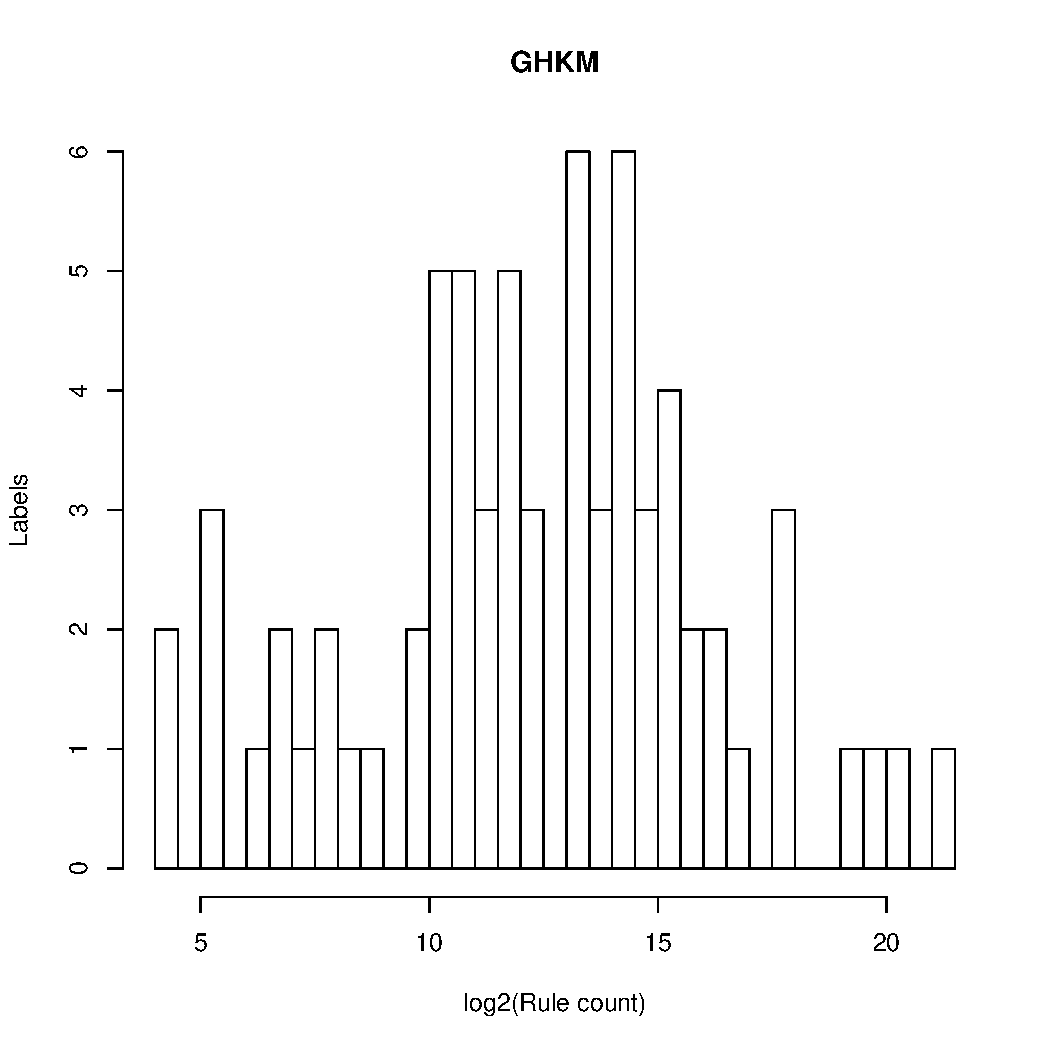
\includegraphics[width=0.5\textwidth]{figures/ghkm}}
%\subfloat[1-best CCG derivations]{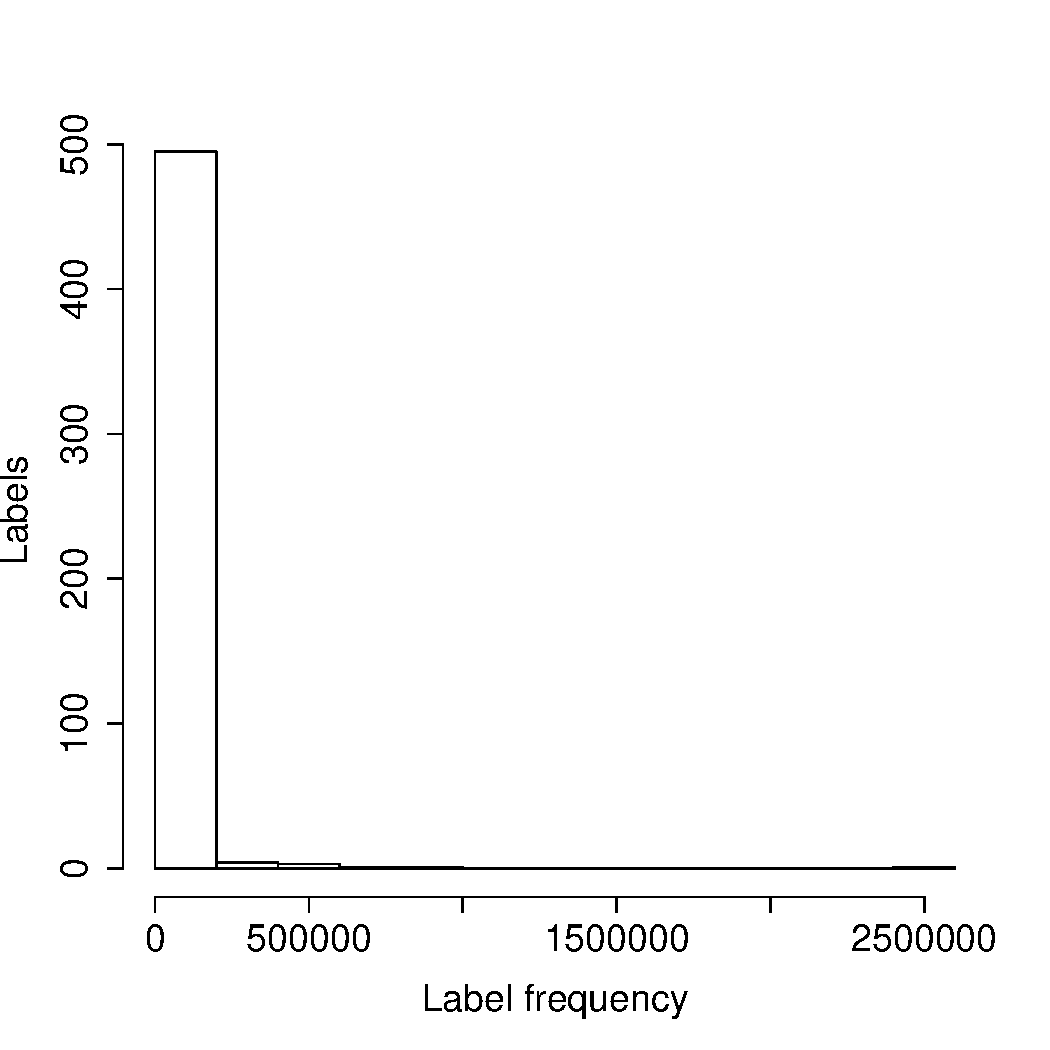
\includegraphics[width=0.5\textwidth]{figures/ccg}} \\
%\subfloat[SAMT]{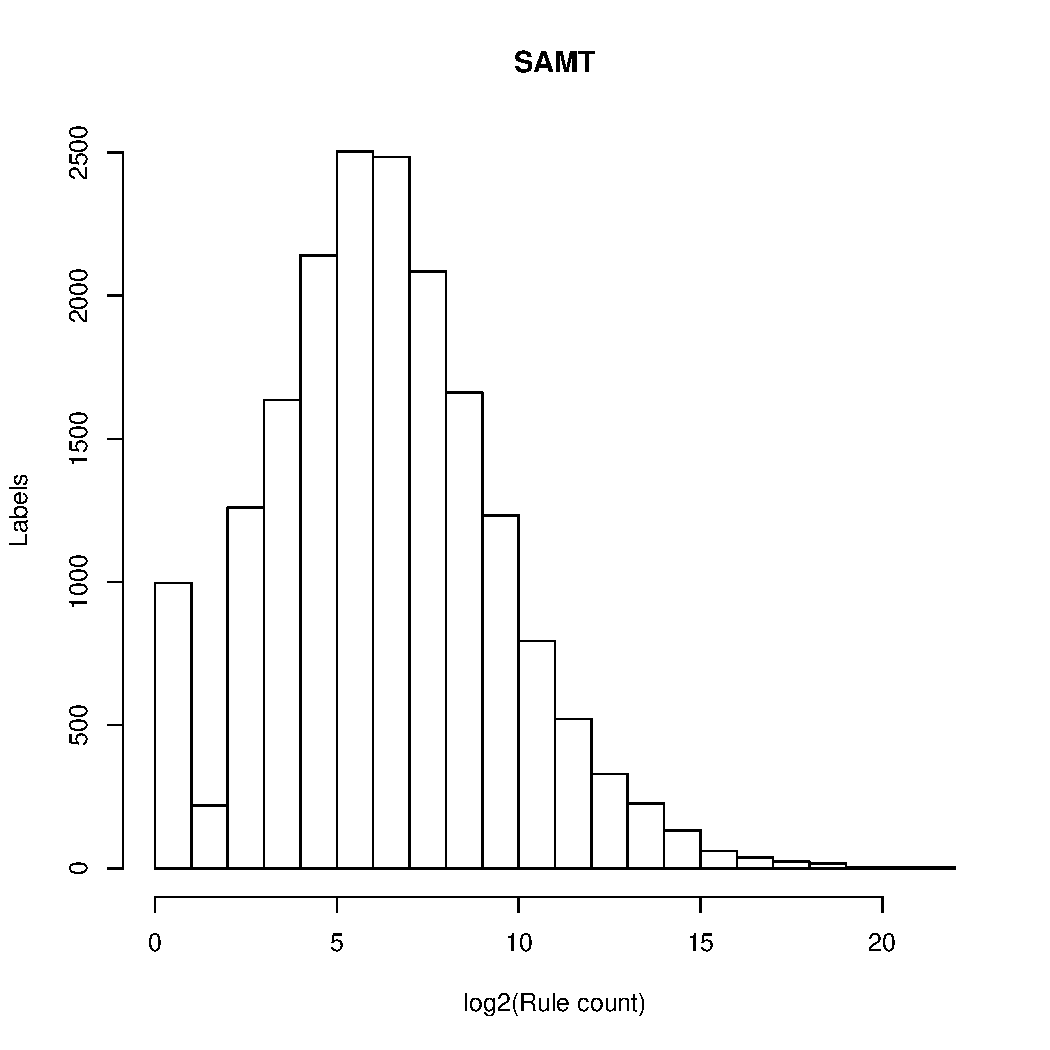
\includegraphics[width=0.5\textwidth]{figures/samt}}
%\subfloat[CCG parse charts\label{fig:hist4}]{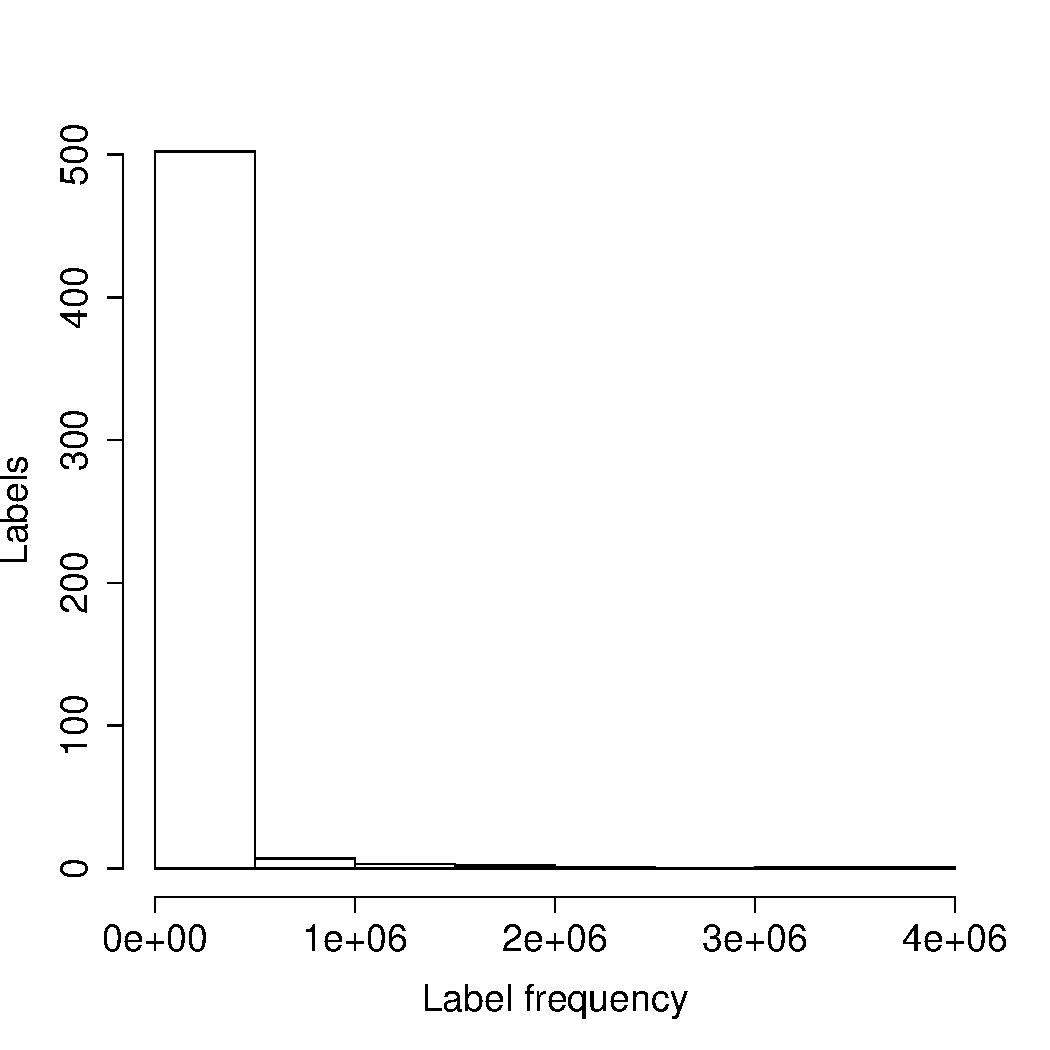
\includegraphics[width=0.5\textwidth]{figures/ccg-auli}}
%\caption{Sparsity of non-terminal symbols. Note the much higher label counts for the SAMT histogram.}
\begin{center}
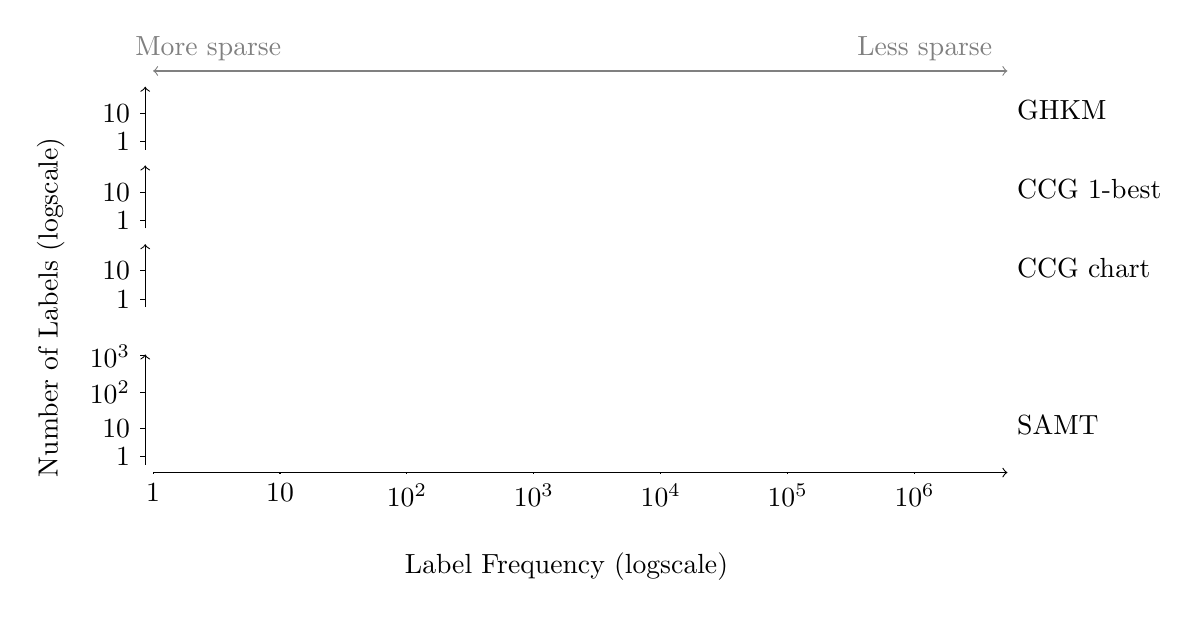
\begin{tikzpicture}[x=0.7cm,y=0.2cm]
    \draw[gray,<->,yshift=1cm] (0,0) -- (15.5,0);
	\node[gray,anchor=south,yshift=1cm] at (1,0) {More sparse};
	\node[gray,anchor=south,yshift=1cm] at (14,0) {Less sparse};
    \draw[->,yshift=-4.1cm] (0,0) -- (15.5,0);
	\foreach \x/\xtext in {0/1,2.30259/10,4.60517/10^2,6.90776/10^3,9.21034/10^4,11.5129/10^5,13.8155/10^6}
		\draw[yshift=-4.1cm] (\x,0) -- (\x,-0.02cm) node[anchor=north] {$\xtext$};
	\draw[->,xshift=-0.1cm] (0,0) -- (0,4);
	\draw[->,xshift=-0.1cm,yshift=-1cm] (0,0) -- (0,4);
	\draw[->,xshift=-0.1cm,yshift=-2cm] (0,0) -- (0,4);
	\draw[->,xshift=-0.1cm,yshift=-4cm] (0,0) -- (0,7);
	\node[anchor=north,yshift=-5cm] at (7.5,0) {Label Frequency (logscale)};
	\foreach \y/\ytext in {0.5/1,2.30259/10}
		\draw[xshift=-0.1cm] (0,\y) -- (-0.1,\y) node[anchor=east] {$\ytext$};
	\foreach \y/\ytext in {0.5/1,2.30259/10}
		\draw[yshift=-1cm,xshift=-0.1cm] (0,\y) -- (-0.1,\y) node[anchor=east] {$\ytext$};
	\foreach \y/\ytext in {0.5/1,2.30259/10}
		\draw[yshift=-2cm,xshift=-0.1cm] (0,\y) -- (-0.1,\y) node[anchor=east] {$\ytext$};
	\foreach \y/\ytext in {0.5/1,2.30259/10,4.60517/10^2,6.90776/10^3}
		\draw[yshift=-4cm,xshift=-0.1cm] (0,\y) -- (-0.1,\y) node[anchor=east] {$\ytext$};
	
	\node[rotate=90,anchor=south,yshift=1cm,xshift=-2cm] at (0,0) {Number of Labels (logscale)};
    \draw[black,thick,ycomb] plot file {data/ghkm.logscale.nts};
    \draw[black,thick,ycomb] plot[yshift=-1cm] file {data/ccg.logscale.nts};
    \draw[black,thick,ycomb] plot[yshift=-2cm] file {data/ccg-auli.logscale.nts};
    \draw[black,thick,ycomb] plot[yshift=-4cm] file {data/samt.logscale.thinned.nts};
	\node[anchor=west,yshift=0.5cm] at (15.5,0) {GHKM};
	\node[anchor=west,yshift=-0.5cm] at (15.5,0) {CCG 1-best};
	\node[anchor=west,yshift=-1.5cm] at (15.5,0) {CCG chart};
	\node[anchor=west,yshift=-3.5cm] at (15.5,0) {SAMT};
\end{tikzpicture}
\caption{Histograms of label frequency for each model, illustrating the sparsity of each model.\label{fig:histogram}}
\end{center}
\end{figure*}


%\begin{figure}[t]
%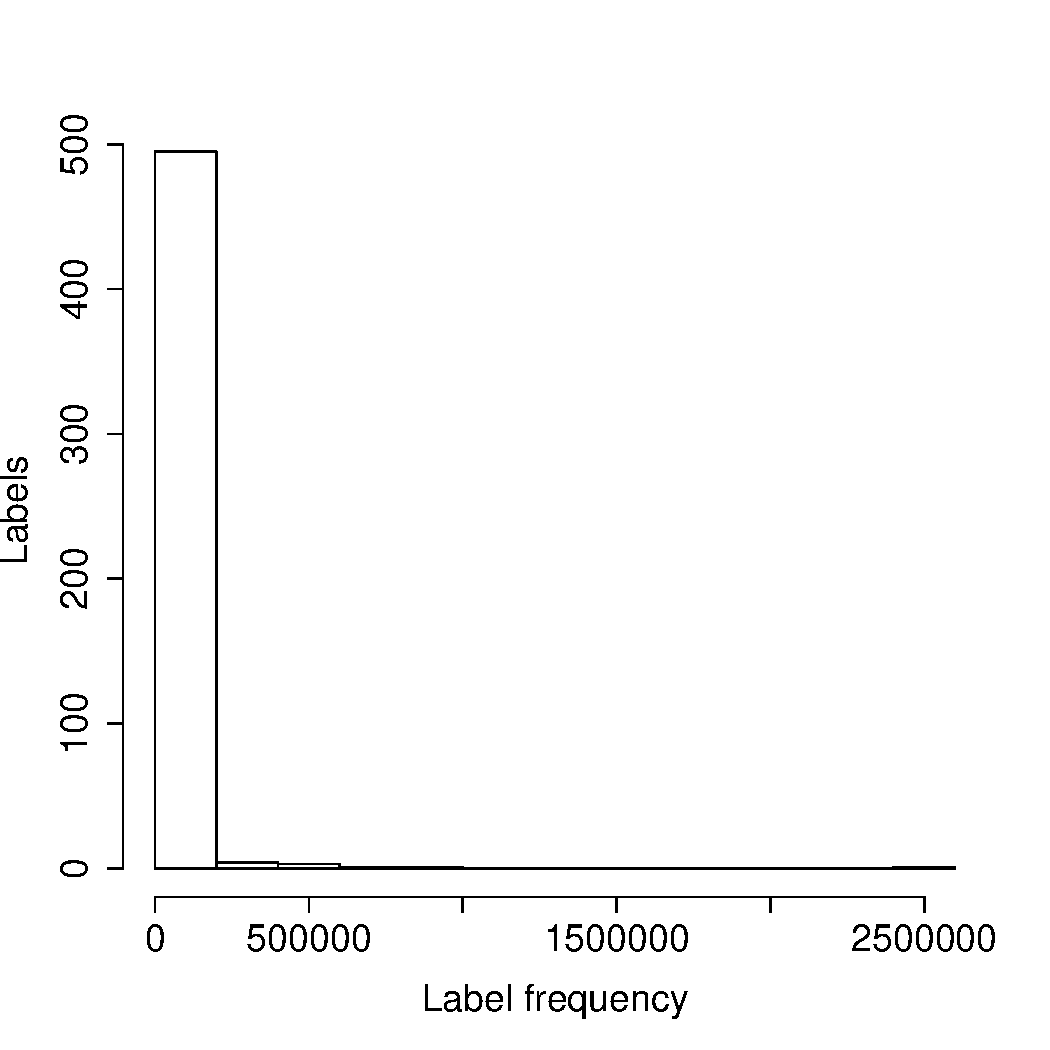
\includegraphics[width=0.5\textwidth]{figures/ccg}
%\caption{Sparsity of non-terminal symbols.}
%\end{figure}

%\begin{figure}[t]
%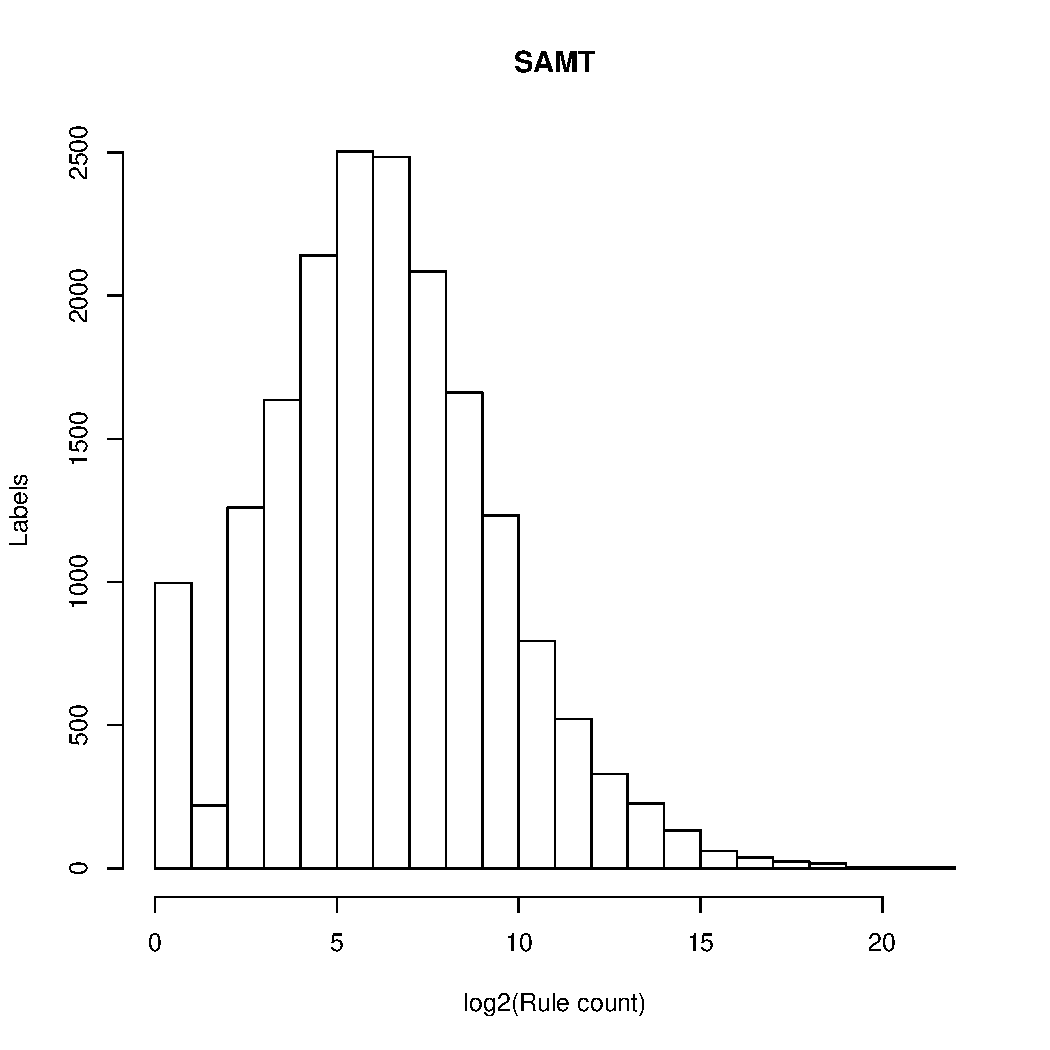
\includegraphics[width=0.5\textwidth]{figures/samt}
%\caption{Sparsity of non-terminal symbols.}
%\end{figure}

%\begin{figure}[t]
%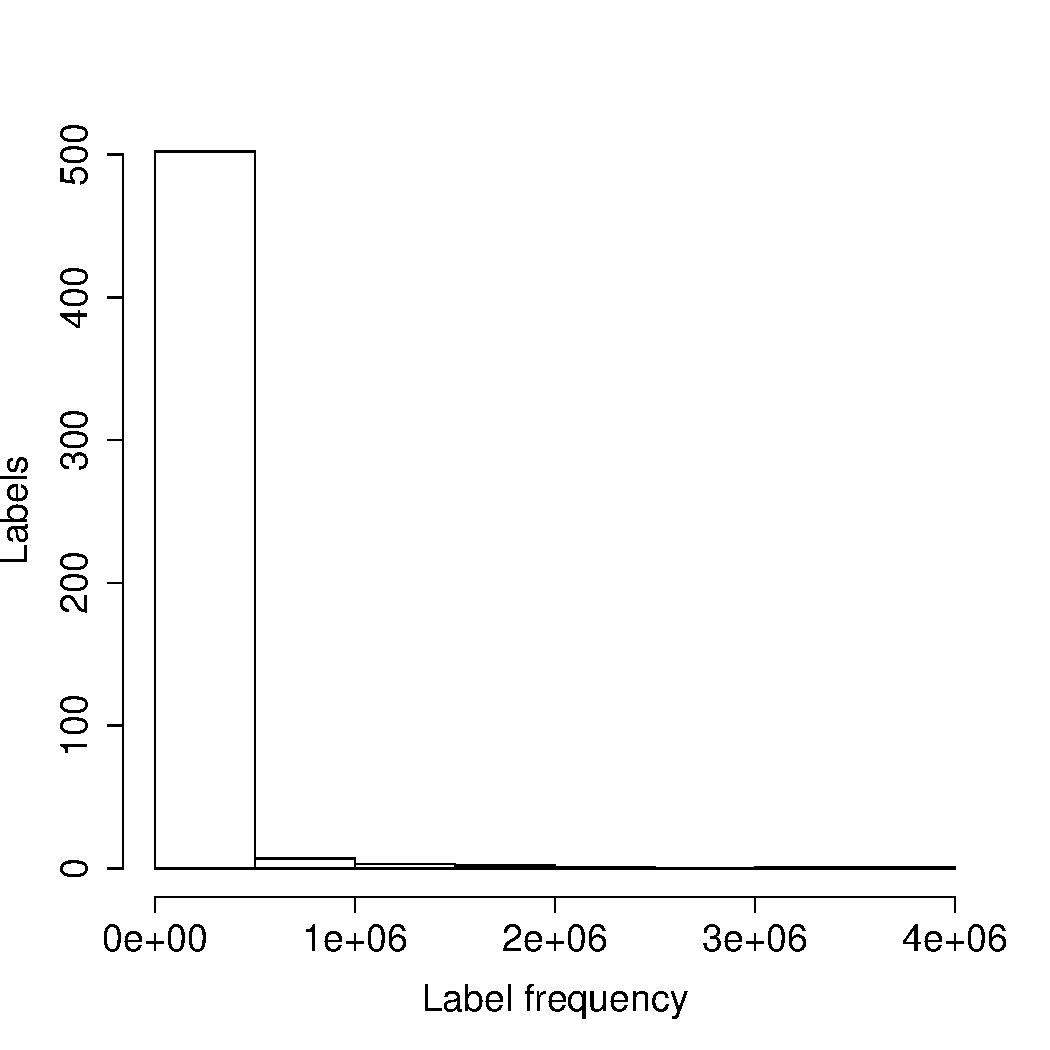
\includegraphics[width=0.5\textwidth]{figures/ccg-auli}
%\caption{Sparsity of non-terminal symbols.\label{fig:hist4}}
%\end{figure}

\subsection{Sparseness of nonterminals}

Examining the histograms in Figure \ref{fig:histogram} gives us a better idea of the non-terminal label sets in our models. In each histogram, the horizontal axis measures the number of times a label appears in the corpus. The height of each bar shows the number of non-terminals that appeared that many times. %The count of rules is scaled logarithmically; therefore, the bar above 0 shows how many non-terminals appear in only one rule in the grammar.

For the phrase structure syntax model, we see there are maybe 20 labels out of 70 that show up on rules less than 1000 times. All the other labels show up on very many rules.

Moving to SAMT, with its heuristically-defined labels, shows a very different story. Not only does the model have over 18,000 non-terminal labels, but thousands of them show up on fewer than 30 rules apiece. If we look at the rare label types, we see that a lot of them are three way concatenations A+B+C that are unlikely to show up a lot in translation. 

\section{Experiments}

\subsection{Data}

We tested our models on an Urdu--English translation task. The training corpus was the National Institute of Standards and Technology Open Machine Translation 2009 Evaluation (NIST Open MT09). According to the MT09 Constrained Training Conditions Resources list\footnote{\url{http://www.itl.nist.gov/iad/mig/tests/mt/2009/MT09_ConstrainedResources.pdf}} this data includes NIST Open MT08 Urdu Resources\footnote{LDC2009E12} and the NIST Open MT08 Current Test Set Urdu--English\footnote{LDC2009E11}. This gives us 202,019 parallel translations, for approximately 2 million words of training data.

\subsection{Experimental design}

We used the scripts included with the Moses MT toolkit \cite{moses} to tokenize and normalize the English data. We used a tokenizer and normalizer developed at the SCALE 2009 workshop \cite{scale09} to preprocess the Urdu data. We used GIZA++ \cite{giza} to perform word alignments.

For phrase structure parses of the English data, we used the Berkeley parser \cite{Petrov-Klein-Inference}. For CCG parses, and for reading labels out of a parse chart, we used the C\&C parser \cite{candc}.

After aligning and parsing the training data, we used the Thrax grammar extractor \cite{joshua3} to extract all of the translation grammars.

We used the same feature set in all the translation grammars. This includes, for each rule $A \to \langle f ; e \rangle$, relative-frequency estimates of the following probabilities:
\begin{itemize}
\item $p(f|A)$, the probability of producing the foreign phrase $f$ given that the generating label is $A$
\item $p(f|e)$, the probability that the foreign phrase $f$ is a translation of the target phrase $e$
\item $p(f|e,A)$, the probability that the foreign phrase $f$ is a translation of $e$ given that the syntactic type is also $A$
\item $p(e|A)$, the probability of producing the target phrase $e$ from the syntactic label $A$
\item $p(e|f)$, the probability that the target phrase $e$ is a translation of the foreign phrase $f$
\item $p(e|f,A)$, the probability that $e$ is a translation of $f$ given that the syntactic type is also $A$
\end{itemize}
The feature set also includes lexical weighting for rules as defined by Koehn et al. \shortcite{koehn-och-marcu-2003} and various binary features as well as counters for the number of unaligned words in each rule.

To train the feature weights we used the Z-MERT implementation \cite{zmert} of the Minimum Error-Rate Training algorithm \cite{mert}.

To decode the test sets, we used the Joshua machine translation decoder \cite{joshua3}.

\subsection{Evaluation criteria}

We measure machine translation performance using the BLEU metric \cite{papineni-bleu}. We also report the translation time for the test set in seconds per sentence. These results are summarized in Table \ref{table:results}.

\begin{table}
\centering
\begin{tabular}{|c|r|r|}
\hline
Model & BLEU & sec./sent. \\
\hline
Hiero & 25.67 (0.9781) & 0.05 \\
Syntax & 27.06 (0.9703) & 3.04 \\
SAMT & 28.06 (0.9714) & 63.48 \\
CCG derivations & 27.3 (0.9770) & 5.24 \\
CCG chart cells & 27.64 (0.9673) & 33.6 \\
\hline
\end{tabular}
\caption{Results of translation experiments on Urdu--English. Higher BLEU scores are better. BLEU's brevity penalty is reported in parentheses.\label{table:results}}
\end{table}

All of the syntactic labeling schemes show an improvement over the Hiero model. Indeed, all the syntactic labeling schemes fall in the range of approximately 27--28 BLEU.

\section{Discussion and Future Work}

Finding an appropriate mechanism to inform phrase-based translation models and their hierarchical variants with linguistic
syntax is a difficult problem that has attracted intense interest, with a variety of promising approaches including
unsupervised clustering \cite{zollmann+vogel:2011:acl}, merging \cite{hanneman+etal:2011}, and selection \cite{hassan+etal:2007:acl}
of labels derived from phrase-structure parse trees very much like those used by our baseline systems. What we find
particularly attractive about CCG is that it naturally assigns linguistically-motivated labels to most spans of a
sentence using a reasonably concise label set, possibility obviating the need for further refinement. Indeed, the 
analytical flexibility of CCG has motivated its increasing use in MT, from applications in language modeling
\cite{birch+etal:2007:wmt,hassan+etal:2007:acl} to more recent proposals to incorporate it into phrase-based
\cite{mehay:2010:proposal} and hierarchical translation systems \cite{auli:2009:first-year}. 

Our new model builds on these past efforts, representing a more fully instantiated model of CCG-based
translation. We have shown that the label scheme allows us to keep many more translation rules than labels based on phrase 
structure syntax, extracting almost as many rules as the SAMT model, but keeping the label set an order of
magnitude smaller, which leads to more efficient translation. This simply scratches the surface of possible
uses of CCG in translation. In future work, we plan to move from a formally context-free to a formally CCG-based
model of translation, implementing combinatorial rules such as application, composition, and type-raising. 

An additional intriguing possibility is to develop a CCG-based model of translation that incorporates semantics,
something that is beginning to attract interest in the translation community \cite{wu+fung:2009:naacl}.
CCG offers a natural interface between syntax and semantics, a property which has been exploited for
a variety of purposes \cite{bos+etal:2004:coling,white+baldridge:2003:enlg,zettlemoyer+collins:2005:uai}.
The key idea is to augment each lexical entry with a semantic value. The use of combinators during parsing then 
naturally builds a semantic representation of a sentence even as it analyzes the syntax.

We can update the function application of Rule \ref{eqn:forward-app} to include semantic annotations:
\begin{equation}
\binaryruleSimple{X/Y:f}{Y:g}{X:fg}
\end{equation}

We anticipate that augmenting CCG-based translation models with semantic representations will be a rich area for future work.

\anonymize{
\section{Acknowledgements*}
Michael Auli, ???, funding sources
}

\bibliographystyle{acl}
\bibliography{ccg}
\end{document}
